\chapter{Integral-Rechnung}
\section{Einf\"uhrung des Integral-Begriffs}
In diesem Kapitel besch\"aftigen wir uns mit der Frage, wie die Fl\"ache zwischen einer Kurve und der
$x$-Achse berechnet werden kann.  Dabei gehen wir davon aus, dass die Kurve durch eine Funktion der
Form $x \mapsto f(x)$ definiert wird.  Um die Dinge konkret zu machen betrachten wir die Funktion 
$x \mapsto x^2$ und fragen, welche Fl\"ache von dieser Kurve und der $x$-Achse im Intervall
$[0,1]$ eingeschlossen wird.  Diese Fl\"ache ist in Abbildung \ref{fig:xhoch2int.eps} 
grau dargestellt.  


\begin{figure}[!h]
  \centering
   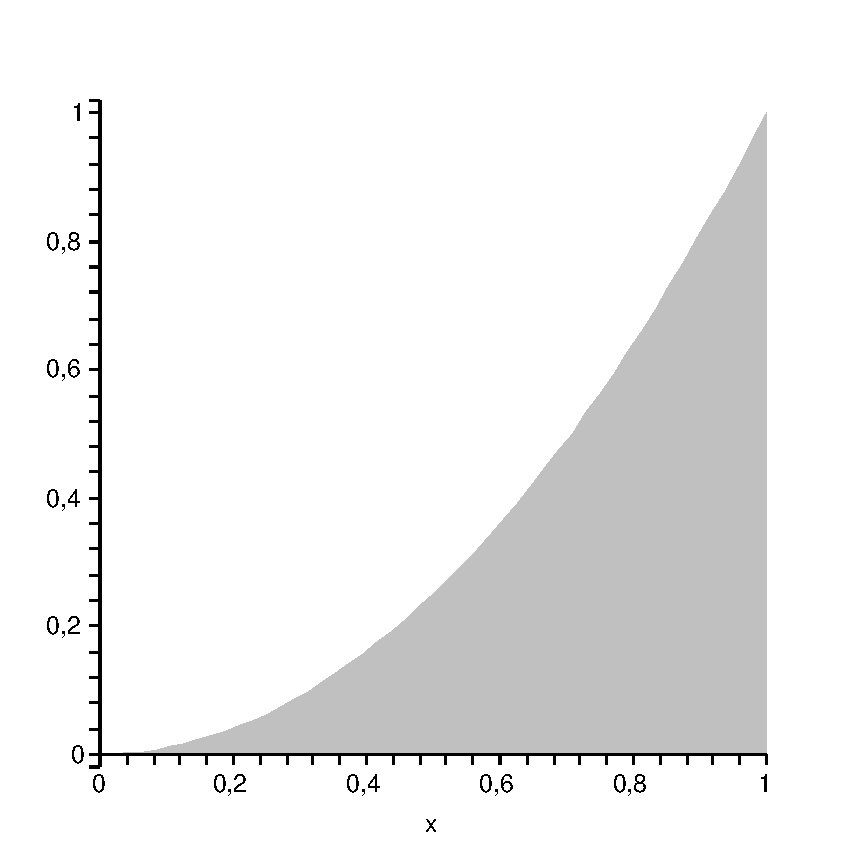
\epsfig{file=Figures/xhoch2int.eps,scale=0.4}
   \caption{Die Fl\"ache unter der Parabel $x \mapsto x^2$ im Intervall $[0,1]$.}
  \label{fig:xhoch2int.eps}
\end{figure}

Wir k\"onnen versuchen, diese Fl\"ache durch sogenannte
\emph{Treppen-Funktionen} zu approximieren.  Eine Treppen-Funktion ist eine Funktion, die
st\"uckweise konstant ist.  Abbildung \ref{fig:xhoch2RiemannRight.eps} auf Seite 
\pageref{fig:xhoch2RiemannRight.eps} zeigt eine Approximation der Funktion $x \mapsto x^2$
durch eine Treppen-Funktion.  In dieser Abbildung haben wir das Intervall $[0,1]$ in 10 gleich
gro{\ss}e Teilintervalle aufgeteilt.  Wollen wir im allgemeinen Fall die Fl\"ache unter eine
Funktion $f$ in einem vorgegebenen Intervall $[a,b]$ berechnen, so 
unterteilen wir das Intervall $[a,b]$ in $n$ Teilintervalle der Form 
\\[0.2cm]
\hspace*{1.3cm}
$\bigl[a + (i-1) \cdot  h, a + i\cdot h \bigr]$ \quad mit $\ds h := \frac{b-a}{n}$ und $i=1,\cdots,n$.
\\[0.2cm]
Um dann die Fl\"ache berechnen zu k\"onnen, approximieren wir diese Fl\"ache
zum einen durch eine Treppen-Funktion, die oberhalb der zu integrierenden Funktion liegt und zum anderen durch eine
Treppen-Funktion, die unterhalb der zu integrierenden Funktion liegt.  Wir nehmen zur
Vereinfachung zun\"achst an, dass die Funktion $f$ monoton steigend ist.
In diesem Fall definieren wir zu einer vorgegebenen Zahl $n$ von Intervallen die obere
Treppen-Funktion $f^\downarrow_{n}(x)$ wie folgt:
\begin{equation}
  \label{eq:treppeOben}
  f^\downarrow_n(x) := f(a + i\cdot h) \quad \mbox{falls}\; 
  x \in  \bigl(a+(i-1)\cdot h,\, a+i\cdot h\bigr)\;\mbox{und}\;i=1,\cdots,n.
\end{equation}
Da wir $f$ als monoton steigend vorausgesetzt haben, gilt 
\\[0.2cm]
\hspace*{1.3cm}
$\forall x \in \bigl( a+(i-1)\cdot h, a+i\cdot h\bigr): f(x) \leq f(a+i\cdot h) = f^\downarrow(x)$,
\\[0.2cm]
die Funktion $f$ liegt also unterhalb der Treppen-Funktion $f^\downarrow$.
Wie die Treppen-Funktion an den Randpunkten der Intervalle $[a+(i-1)\cdot h, a+i\cdot h]$ definiert
wird, ist unwichtig.  Abbildung \ref{fig:xhoch2RiemannRight.eps} zeigt die Funktion 
$f(x) = x^2$ und die zugeh\"orige Treppen-Funktion $f^\downarrow_{10}(x)$.  Die Fl\"ache unter
einer solchen Treppen-Funktion kann leicht berechnet werden:  Schreiben wir
\\[0.2cm]
\hspace*{1.3cm}
$\ds \int_a^b f(x) \,\dr x$
\\[0.2cm] 
f\"ur die Fl\"ache unter einer Funktion $f$ in dem Intervall $[a,b]$, so gilt f\"ur die
Treppen-Funktion $f^\downarrow_{n}$ offenbar
\begin{equation}
  \label{eq:intOber}
  \int_a^b f^\downarrow_n(x) \,\dr x = \sum\limits_{i=1}^n f(a+i\cdot h)\cdot h
\end{equation}
denn die Fl\"ache eines Rechtecks berechnet sich als das Produkt von Breite und H\"ohe.  Die
H\"ohe des Rechtecks im $i$-ten Teilintervall hat den Wert $f(a + i\cdot h)$ und die Breite
des Teilintervalls ist $h$.

\begin{figure}[!t]
  \centering
   \epsfig{file=Figures/xhoch2RiemannRight.eps,scale=0.5}
   \caption{Die Fl\"ache unter der Parabel $x \mapsto x^2$ im Intervall $[0,1]$.}
  \label{fig:xhoch2RiemannRight.eps}
\end{figure}

Genau wie wir die Fl\"ache unter der Funktion $f$ von oben approximieren k\"onnen, k\"onnen wir
diese Fl\"ache auch von unten approximieren. Die dazu notwendige Treppen-Funktion
$f^\uparrow_n(x)$ definieren wir analog zu Gleichung (\ref{eq:treppeOben})
\begin{equation}
  \label{eq:treppeUnten}
  f^\uparrow_n(x) = f(a + (i-1)\cdot h) \quad \mbox{falls}\; x \in (a+(i-1)\cdot h, a+i\cdot h),
\end{equation}
wir werten also diesmal in jedem Intervall die Funktion $f$ am linken Eckpunkt aus,
denn dort ist die Funktion $f$ am kleinsten, da wir vorausgesetzt haben, dass
die Funktion $f$ monoton steigend ist.
F\"ur diese Treppen-Funktion berechnet sich die Fl\"ache nach der Formel
\begin{equation}
  \label{eq:intUnter}
  \int_a^b f^\uparrow_n(x) \,\dr x = \sum\limits_{i=1}^{n} f\bigl(a+(i-1)\cdot h\bigr)\cdot h
  = \sum\limits_{i=0}^{n-1} f(a+i\cdot h)\cdot h.
\end{equation}
F\"ur die Fl\"ache, die zwischen der Funktion $f$ und der $x$-Achse liegt, haben wir insgesamt
die Absch\"atzung
\\[0.2cm]
\hspace*{1.3cm}
$\ds\sum\limits_{i=0}^{n-1} f(a+i\cdot h)\cdot h \leq \int_a^b f(x) \,\dr x \leq \sum\limits_{i=1}^{n} f(a+i\cdot h)\cdot h$ 
\\[0.2cm]
gefunden.  Die linke Summe bezeichnen wir als \emph{Unter-Summe}, die Summe auf der
rechten Seite der Ungleichungskette nennen wir \emph{Ober-Summe}.
Wir k\"onnen hoffen, dass f\"ur wachsende Werte von $n$ die Werte von Ober-Summe und
Unter-Summe gegen den selben Grenzwert konvergieren.  Dazu berechnen wir zun\"achst die
Differenz dieser beiden Summen:
\\[0.2cm]
\hspace*{1.3cm}
$
\begin{array}{cl} 
    & \ds \sum\limits_{i=1}^{n} f(a+i\cdot h)\cdot h - \sum\limits_{i=0}^{n-1} f(a+i\cdot h)\cdot h \\[0.4cm]
 =  & \ds f(a+n\cdot h)\cdot h - f(a)\cdot h  \\[0.1cm]
 =  & \ds \biggl(f\Bigl(a+n\cdot \frac{b-a}{n}\Bigr) - f(a)\biggr)\cdot  \frac{b-a}{n}  \\[0.3cm]
 =  & \ds \Bigl(f(a+ b-a) - f(a)\Bigr)\cdot  \frac{b-a}{n}  \\[0.3cm]
 =  & \ds \Bigl(f(b) - f(a)\Bigr)\cdot  \frac{b-a}{n}  \\[0.3cm]
{\longrightarrow \atop {n \rightarrow \infty}} & 0
\end{array}
$
\\[0.3cm]
Damit ist klar, dass bei einer monoton steigenden Funktion die Ober-Summe f\"ur eine
wachsende Zahl $n$ von Intervallen gegen den 
selben Wert konvergiert wie die Unter-Summe.  Daher definieren wir
\begin{equation}
  \label{eq:integral}
  \int_a^b f(x) \,\dr x := \lim\limits_{n\rightarrow \infty} \sum\limits_{i=1}^n f\Bigl(a + i
  \cdot \frac{b-a}{n}\Bigr) \cdot \frac{b-a}{n}
\end{equation}
Diesen Grenzwert nennen wir auch das \emph{Integral} von $f$ in dem Intervall $[a,b]$.
Die so gegebene Definition ist zun\"achst nur f\"ur monoton wachsende Funktionen schl\"ussig,
aber es ist offensichtlich, dass das Integral f\"ur monoton fallende Funktionen auf die
selbe Weise berechnet werden kann.  Ist nun eine Funktion $f$ in dem Intervall $f$ weder
monoton fallend noch monoton steigend, so k\"onnen wir versuchen, dass Intervall so in
Teilintervalle aufzuspalten, dass $f$ in jedem Teilintervall monoton fallend oder monoton
steigend ist.  Da wir auf jedem dieser Teilintervalle das Integral nach der Formel 
(\ref{eq:integral}) berechnen k\"onnen, k\"onnen wir dann auch insgesamt das Integral nach
dieser Formel berechnen.

\exercise
Berechnen Sie das Integral 
\\[0.2cm]
\hspace*{1.3cm}
$\dint{0}{b} x^2\, \dr x$
\\[0.2cm]
nach der in (\ref{eq:integral}) angegebenen Formel.
\vspace*{0.2cm}

\noindent
\textbf{Hinweis:}  Es gilt
\\[0.2cm]
\hspace*{1.3cm}
$\ds \sum\limits_{i=1}^n i^2 = \frac{n}{6} \cdot (n + 1) \cdot (2 \cdot n + 1)$.
\eox

\begin{Definition}[Integral]
  Ist $f:[a,b] \rightarrow \mathbb{R}$ eine Funktion, so dass der Grenzwert 
\\[0.2cm]
\hspace*{1.3cm}
$\ds\lim\limits_{n\rightarrow \infty} \sum\limits_{i=1}^n f\Bigl(a + i \cdot  \frac{b-a}{n}\Bigr) \cdot \frac{b-a}{n}$
\\[0.2cm]
existiert, so nennen wir $f$ \blue{integrierbar} und definieren das \blue{Integral} von $f$
in dem Intervall $[a,b]$ als 
  \\[0.2cm]
  \hspace*{1.3cm}
  \colorbox{red}{\colorbox{orange}{\framebox{$\dint{a}{b} f(x) \,\dr x = 
   \lim\limits_{n\rightarrow \infty} \sum\limits_{i=1}^n f\Bigl(a + i \cdot \frac{b-a}{n}\Bigr) \cdot \frac{b-a}{n}
  $.}}}  \eod
\end{Definition}

\noindent
Der so eingef\"uhrte Integral-Begriff hat folgende Eigenschaften:
\begin{enumerate}
\item \blue{Linearit\"at:} Sind $f$ und $g$ zwei Funktionen, so dass
      das Integral \"uber $f$ bzw.~$g$ in dem Inter\-vall $[a,b]$ definiert ist
      und sind $\alpha,\beta \in\mathbb{R}$,
      so ist auch das Integral der Funktion
      \\[0.2cm]
      \hspace*{1.3cm} $x \mapsto \alpha\cdot f(x) + \beta\cdot g(x)$ \\[0.2cm]
      definiert und es gilt 
      \\[0.2cm]
      \hspace*{1.3cm}
      $\ds\int_a^b \alpha\cdot f(x) + \beta\cdot g(x)\,\dr x = \alpha\cdot \int_a^b f(x)\,\dr x + \beta\cdot \int_a^b g(x)\,\dr x$.
      \\[0.2cm]
      Diese Eigenschaft folgt aus der Tatsache, dass einerseits sowohl die Summe als auch das
      Produkt zweier konvergenter Folgen wieder konvergent sind und das andererseits im Falle
      konvergenter Folgen der Grenzwert sowohl mit der Summe als auch mit dem Produkt vertauscht
      werden kann.
\item \blue{Monotonie:}  Sind $f$ und $g$ zwei Funktionen, so dass
      das Integral \"uber $f$ und  $g$ in dem Intervall $[a,b]$ definiert ist, so gilt: 
      \\[0.2cm]
      \hspace*{1.3cm}
      $\ds\Bigl(\forall x \in [a,b]: f(x) \leq g(x)\Bigr) \;\Rightarrow\;
       \int_a^b f(x)\, \dr x \,\leq\, \int_a^b g(x)\, \dr x$.
      \\[0.2cm] 
      Auch diese Eigenschaft folgt aus der entsprechenden Eigenschaft konvergenter Folgen.
\end{enumerate}


\begin{Satz}[Mittelwert-Satz der Integral-Rechnung] \hspace*{\fill} \\
Es sei $f:[a,b] \rightarrow \mathbb{R}$ eine stetige Funktion. Dann existiert ein $\xi \in [a,b]$, so dass gilt:
\\[0.2cm]
\hspace*{1.3cm}
\colorbox{red}{\colorbox{orange}{\framebox{$\ds\int_a^b f(x) \,\dr x = f(\xi) \cdot  (b - a)$.}}}
\end{Satz}

\noindent
\textbf{Beweis}: Da die Funktion $f$ stetig ist, nimmt $f$ auf dem Intervall $[a,b]$ ein
Minimum und ein Maximum in den Punkten $x_{min}$ und $x_{max}$ an.  Dann gilt 
\\[0.2cm]
\hspace*{1.3cm}
$\forall x \in [a,b]: f\bigl(x_{min}\bigr) \leq f(x) \leq f\bigl(x_{max}\bigr)$.
\\[0.2cm]
Aufgrund der Monotonie des Integral-Operators folgt daraus sofort 
\\[0.2cm]
\hspace*{1.3cm}
$
\begin{array}{cl} 
                & \dint{a}{b} f\bigl(x_{min}\bigr)\, \dr x \leq \int_a^b f(x)\, \dr x \leq \int_a^b f\bigl(x_{max}\bigr)\,\dr x \\[0.3cm]
\Leftrightarrow & \ds f\bigl(x_{min}\bigr) \cdot  (b-a) \leq \int_a^b f(x)\, \dr x \leq f\bigl(x_{max}\bigr)\cdot (b-a) \\[0.3cm]
\Leftrightarrow & \ds f\bigl(x_{min}\bigr) \leq \frac{1}{b-a} \cdot \int_a^b f(x)\, \dr x \leq f\bigl(x_{max}\bigr) \\[0.3cm]
\end{array}
$
\\[0.2cm]
Die obige Ungleichungskette zeigt, dass 
\\[0.2cm]
\hspace*{1.3cm}
 $\ds \frac{1}{b-a} \cdot \int_a^b f(x)\, \dr x\; \in \bigl[f(x_{min}), f(x_{max})\bigr]$ \\[0.2cm]
gilt.  
Aufgrund des Zwischenwert-Satzes f\"ur stetige Funktionen (Satz \ref{satz:zws-stetig} auf Seite
\pageref{satz:zws-stetig}) nimmt die stetige Funktion $f$ jeden Wert in dem  
Intervall $\bigl[f\bigl(x_{min}\bigr), f\bigl(x_{max}\bigr)\bigr]$ an.  
Also gibt es ein $\xi \in [a,b]$, so dass 
\\[0.2cm]
\hspace*{1.3cm}
$f(\xi) = \ds \frac{1}{b-a} \cdot \int_a^b f(x)\, \dr x$
\\[0.2cm]
gilt und dass ist \"aquivalent zu 
\\[0.2cm]
\hspace*{1.3cm}
$\ds f(\xi) \cdot  (b- a) = \int_a^b f(x)\, \dr x$. \hspace*{\fill} $\Box$
\vspace*{0.3cm}

\noindent
Der Mittelwert-Satz versetzt uns in die Lage, einen Zusammenhang zwischen
Differential-Rechnung und Integral-Rechnung herzustellen.

\begin{Satz}[Ableitung von Integralen] \lb
  \label{satz:ableitungInt}
  Die Funktion $f:[a,b] \rightarrow \mathbb{R}$ sei stetig.  Definieren wir f\"ur 
  $x \in [a,b]$ die Funktion  $F:[a,b] \rightarrow \mathbb{R}$ durch 
  \\[0.2cm]
  \hspace*{1.3cm}
  $\ds F(x) := \int_a^x f(t)\, \dr t$,
  \\[0.2cm]
  so ist die Funktion $F$ im Intervall $[a,b]$ differenzierbar und es gilt 
  \\[0.2cm]
  \hspace*{1.3cm} $\df F(x) = f(x)$.
\end{Satz}

\noindent
\textbf{Beweis}: Es gilt
\\[0.3cm]
\hspace*{1.3cm}
$
\begin{array}[t]{cll}  

   &\ds \df F(x) \\[0.3cm]
 = &\ds  \lim\limits_{h\rightarrow 0} \frac{F(x+h) - F(x)}{h} \\[0.3cm]
 = &\ds \lim\limits_{h\rightarrow 0} \ds\frac{\int_a^{x+h} f(t)\, \dr t - \int_a^x f(t)\, \dr t}{h} &
      \mbox{nach Definition von $F$} \\[0.3cm]
 = &\ds \lim\limits_{h\rightarrow 0} \ds\frac{1}{h}\int_{x}^{x+h} f(t)\, \dr t \\[0.5cm]
 = &\ds \lim\limits_{h\rightarrow 0} \ds\frac{1}{h} \cdot  (x+h - x) \cdot   f(\xi_h) &
      \mbox{nach dem Mittelwertsatz f\"ur ein $\xi_h\in[x, x+h]$} \\[0.5cm]
 = &\ds \lim\limits_{h\rightarrow 0} \ds f(\xi_h) \\[0.3cm]
 = & \ds f(x) & \mbox{wegen $\xi_h \in [x, x+h]$}.
\end{array}
$
\\[0.3cm]
Damit ist die Behauptung bewiesen. \hspace*{\fill} $\Box$

\remark
Der letzte Satz zeigt uns, dass der Differentiations-Operator
\\[0.2cm]
\hspace*{1.3cm}
$\ds\frac{\textrm{d}\,\;}{\textrm{d}x} := \left(f \mapsto \frac{\textrm{d}f}{\textrm{d}x} \right)$ 
\\[0.2cm]
zu dem Integral-Operator
\\[0.2cm]
\hspace*{1.3cm}
$\ds\int_{a}^x \cdot \;\dr t := \left(f \mapsto \int_a^x f(t) \, \dr t\right)$ 
\\[0.2cm]
invers ist: Wenden wir auf eine Funktion zun\"achst den
Integral-Operator an und wenden wir dann auf die resultierende Funktion den
Differentiations-Operator an, so erhalten wir wieder die urspr\"ungliche Funktion:
\\[0.2cm]
\hspace*{1.3cm}
\colorbox{red}{\colorbox{orange}{\framebox{$\ds \frac{\dr\;}{\dr x} \int_a^x f(t)\,\dr t = f(x)$.}}}
\\[0.2cm]
Diese Aussage
l\"asst sich im Wesentlichen auch umkehren.  Diese Umkehrung ist der Hauptsatz der Differential- und
Integral-Rechnung.  Bevor wir diesen Satz in Angriff nehmen k\"onnen, ben\"otigen wir noch eine Definition.
\pagebreak

\begin{Definition}[Stamm-Funktion] \lb
Ist $f:[a,b] \rightarrow \mathbb{R}$ eine Funktion, so nennen wir die Funktion  $F:[a,b]\rightarrow\mathbb{R}$ 
eine \blue{Stamm-Funktion} von $f$, falls $F$ differenzierbar ist und 
\\[0.2cm]
\hspace*{1.3cm} $\df F(x) = f(x)$
\\[0.2cm]
gilt.  In diesem Fall schreiben wir auch  $\ds F(x) = \int f(x) \, \dr x$.
Der Ausdruck $\ds\int f(x) \, \dr x$ wird als \blue{unbestimmtes}
\blue{Integral} bezeichnet. \eod
\end{Definition}

Die Schreibweise $F(x) = \int f(x) \, \dr x$ ist problematisch, denn die Stamm-Funktion einer
gegebenen Funktion ist nicht eindeutig.  Ist $F(x)$ eine Stamm-Funktion von $f(x)$ und
definieren wir die Funktion $G$ durch $G(x) := F(x) + c$ f\"ur eine beliebige Konstante $c$,
so ist nat\"urlich auch $G(x)$ eine Stamm-Funktion von $f$, denn es gilt
\\[0.2cm]
\hspace*{1.3cm}
$\df G(x) = \df F(x) + \df c = f(x) + 0 = f(x)$.
\\[0.2cm]
Umgekehrt gilt, dass zwei verschiedene Stamm-Funktionen zu einer Funktion $f$ sich nur um
eine Konstante unterscheiden.  Dies sehen wir wie folgt: Angenommen, $F_1$ und $F_2$ seien
zwei Stamm-Funktionen einer Funktion $f$, es gelte also 
\\[0.2cm]
\hspace*{1.3cm}
$\df{F_1}(x) = f(x)$ \quad und \quad $\df{F_2}(x) = f(x)$.
\\[0.2cm]
Dann definieren wir die Funktion $H$ als $H(x) := F_1(x) - F_2(x)$.  Damit gilt
\\[0.2cm]
\hspace*{1.3cm}
$\df H(x) = \df{F_1}(x) - \df{F_2}(x) = f(x) - f(x) = 0$.
\\[0.2cm]
Nach Lemma \ref{lemma:0_ableitung} gibt es nun eine Konstante $c$, so dass $H(x) = c$ gilt.
Daraus folgt dann
\\[0.2cm]
\hspace*{1.3cm}
$F_1(x) - F_2(x) = c$, \quad also \quad $F_1(x) = F_2(x) + c$
\\[0.2cm]
und das hei{\ss}t gerade, dass sich die beiden Stamm-Funktionen $F_1$ und $F_2$ nur um eine Konstante
unterscheiden.   

Sie fragen sich vermutlich, warum wir bei einer Stamm-Funktion das Integral-Zeichen verwenden.
Der Hauptsatz der Differential- und Integral-Rechnung gibt darauf eine Antwort.  Gleichzeitig ist
dieser Satz das zentrale Ergebnis dieser Vorlesung.  Historisch wurde dieser Satz unabh\"angig sowohl
von \href{https://en.wikipedia.org/wiki/Gottfried_Wilhelm_Leibniz}{Gottfried Wilhelm Leibniz} als
auch von \href{https://en.wikipedia.org/wiki/Isaac_Newton}{Issac Newton} gefunden.  Die Entdeckung
dieses Satzes war f\"ur die Analysis von  fundamentaler Bedeutung, denn dieser Satz erm\"oglicht die
Berechnung vieler Integrale.

\begin{Satz}[Hauptsatz der Differential- und Integral-Rechnung] \hspace*{\fill} \\
 Die Funktion $f:[a,b] \rightarrow\mathbb{R}$ sei stetig, $F:[a,b] \rightarrow\mathbb{R}$
sei eine Stamm-Funktion von $f$ und es gelte $u,v\in[a,b]$.  Dann gilt
\\[0.2cm]
\hspace*{1.3cm}
\colorbox{red}{\colorbox{orange}{\framebox{$\dint{u}{v} f(x)\,\dr x = F(v) - F(u)$.}}}  
\end{Satz}

\noindent
\textbf{Beweis}: Definieren wir die Funktion $G(x)$ durch 
\\[0.2cm]
\hspace*{1.3cm}
$\ds G(x) := \int_a^x f(t)\, \dr t$ \quad f\"ur alle $x\in[a,b]$,
\\[0.2cm]
so besagt Satz \ref{satz:ableitungInt}, dass die Funktion $G$ eine Stamm-Funktion der
Funktion $f$ ist.  Ist nun $F$ eine beliebige weitere Stamm-Funktion von $f$, so haben wir
gerade gesehen, dass die Stamm-Funktionen $G$ und $F$ sich nur um eine Konstante $c$
unterscheiden k\"onnen, es gilt also
\\[0.2cm]
\hspace*{1.3cm}
$F(x) = G(x) + c$.
\\[0.2cm]
Damit haben wir 
\\[0.2cm]
\hspace*{1.3cm}
$
\begin{array}[t]{lcl}
  F(v) - F(u) & = & G(v) + c - \bigl(G(u) + c\bigr) \\[0.2cm]
              & = & G(v) - G(u)                     \\[0.2cm]
              & = & \ds\int_a^v f(t)\, \dr t - \int_a^u f(t)\, \dr t \\[0.3cm]
              & = & \ds\int_u^v f(t)\, \dr t. \hspace*{9cm} \Box  
\end{array}
$
\vspace*{0.3cm}

\noindent
Der letzte Satz gibt Anlass zu einer Schreibweise.  F\"ur eine Funktion $F$  definieren wir
\\[0.2cm]
\hspace*{1.3cm}
$F(x) \Big|_u^v := F(v) - F(u)$.
\\[0.2cm]
Den letzten Satz k\"onnen wir eine wichtige Schlussfolgerung ziehen:  Ist $f:[a,b] \rightarrow\mathbb{R}$
eine differenzierbare Funktion, so ist $f$ offenbar eine Stamm-Funktion der Funktion $f'(x)$.
Also gilt:
\begin{equation}
  \label{eq:hauptsatzKorollar}
  \colorbox{red}{\colorbox{orange}{\framebox{$\ds\int_u^v f'(x)\,\dr x = f(v) - f(u) = f(x)\Big|_u^v$}}}
\end{equation}
Dies zeigt uns, dass der Integral-Operator in gewisser Weise zum Differential-Operator invers ist.

\section{Regeln zur Berechnung von Integralen}
Der Hauptsatz der Differential- und Integral-Rechnung erm\"oglicht es, Regeln zur Berechnung
von Integralen aufzustellen.  Tabelle \ref{tab:integrale} zeigt die Stamm-Funktionen der
wichtigsten Funktionen.  Um diese Tabelle zu verifizieren reicht es aus, die in der rechten
Spalte der Tabelle angegebene Funktion nach $x$ zu differenzieren.
Wir f\"uhren dies exemplarisch f\"ur den Eintrag $\ln(x)$ vor.  Es gilt
\\[0.3cm]
\hspace*{1.3cm}
$
\begin{array}[t]{lcll}  
\dfo \bigl( x\cdot \ln(x) - x\bigr) & = & \dfo \bigl( x\cdot \ln(x) \bigr) - \dfo x \\[0.3cm] 
 & = &\ds 1 \cdot  \ln(x) + x \cdot  \frac{1}{x} - 1 & (\mbox{Produkt-Regel}) \\[0.2cm]
 & = &\ds \ln(x) + 1 - 1  \\[0.2cm]
 & = & \ds \ln(x) \\
\end{array}
$
\\[0.3cm]
Damit ist gezeigt, dass $\ds\int \ln(x)\;\dr x = x\cdot \ln(x) - x$ gilt.  Die \"ubrigen Eintr\"age der
Tabelle k\"onnen auf \"ahnliche Weise verifiziert werden.

\begin{table}[h]
  \centering
  \begin{tabular}[t]{|l|l|}
    \hline
    Funktion $f(x)$ & Stamm-Funktion $\ds \rule[-12pt]{0pt}{30pt}\int\!\! f(x) \, \dr x$ \\
    \hline
    \hline
    $x^\alpha$ mit $\alpha\not= -1$ & \rule[-12pt]{0pt}{30pt} $\ds \frac{1}{\alpha + 1}\cdot x^{\alpha + 1}$ \\
    \hline
    $\ds \frac{1}{x} $ & \rule[-12pt]{0pt}{30pt} $\ln\bigl(|x|\bigr)$ \\
    \hline
    $\exp(x)$                      & \rule[-6pt]{0pt}{18pt} $\exp(x)$ \\
    \hline
    $\sin(x)$                      & \rule[-6pt]{0pt}{18pt} $-\cos(x)$ \\
    \hline
    $\cos(x)$                      & \rule[-6pt]{0pt}{18pt} $\sin(x)$ \\
    \hline
    $\tan(x) $ & \rule[-6pt]{0pt}{18pt} $-\ln\bigl(|\cos(x)|\bigr)$ \\
    \hline
    $\ln(x)$ & \rule[-6pt]{0pt}{18pt} $x\cdot \ln(x) - x$ \\
    \hline
    $\ds \frac{1}{1+x^2}$ & \rule[-12pt]{0pt}{30pt} $\arctan(x)$ \\
    \hline
    $\ds \frac{1}{\sqrt{1-x^2}} $ & \rule[-14pt]{0pt}{30pt} $\arcsin(x)$ \\
    \hline
    $\ds \frac{1}{\sqrt{1+x^2}} $ & \rule[-14pt]{0pt}{30pt} $ \ln  \left( x+\sqrt {1+{x}^{2}} \right) $ \\
    \hline
    $\arctan(x)$ & \rule[-12pt]{0pt}{30pt} $\ds x\cdot \arctan(x) -\frac{1}{2}\cdot \ln\bigl( 1+{x}^{2} \bigr)$ \\
    \hline
  \end{tabular}
  \caption{Tabelle einiger Integrale}
  \label{tab:integrale}
\end{table}
Bemerkenswert ist vielleicht noch die Stamm-Funktion der Funktion $\ds x \mapsto \frac{1}{x}$:
F\"ur $x>0$ gilt 
sicher 
\\[0.2cm]
\hspace*{1.3cm}
$\dfo \ln(x) = \frac{1}{x}$
\\[0.2cm]
Au{\ss}erdem gilt nach der Ketten-Regel f\"ur $x < 0$ 
\\[0.2cm]
\hspace*{1.3cm}
$\dfo \ln(-x) = -1 \cdot  \frac{1}{-x} = \frac{1}{x}$.
\\[0.2cm]
Diese beiden Gleichungen k\"onnen wir zu 
\\[0.2cm]
\hspace*{1.3cm}
$\dfo \ln\bigl(|x|\bigr) = \frac{1}{x}$
\\[0.2cm]
zusammen fassen und folglich haben wir
\\[0.2cm]
\hspace*{1.3cm}
 $\bint \frac{1}{x}\,\dr x = \ln\bigl(|x|\bigr)$.
\\[0.2cm]
Wir k\"onnen die einzelnen Eintr\"age der Tabelle zwar durch Differenzieren leicht
verifizieren, aber dabei bleibt die Frage offen, wie die Eintr\"age dieser Tabelle gefunden
wurden.  Wir stellen jetzt einige S\"atze auf, mit deren Hilfe wir Stamm-Funktionen
gegebener Funktionen berechnen k\"onnen.  Wir erhalten diese S\"atze indem wir die
Regeln, die wir zur Differenzierung aufgestellt haben, umdrehen.  


\subsection{Die Substitutions-Regel}
Wir beginnen mit der Ketten-Regel. Es gilt:
\\[0.3cm]
\hspace*{1.3cm}
$\dfo h(f(x)) = f'(x) \cdot  h'(f(x))$
\\[0.3cm]
Also ist die Funktion $x \mapsto h(f(x))$ eine Stamm-Funktion der Funktion $x \mapsto f'(x) \cdot  h'(f(x))$.
Nach dem Hauptsatz gilt dann 
\begin{equation}
  \label{eq:subst0}
  \int_a^b f'(x) \cdot  h'(f(x))\, \dr x  =  h\bigl(f(b)\bigr) - h\bigl(f(a)\bigr)
\end{equation} 
Wir definieren nun $g(x) := h'(x)$.  Dann ist $h$ eine Stamm-Funktion der Funktion $g$, es
gilt also $h(x) = \int g(x)\, \dr x \,+\, d$ , was wir nach dem Hauptsatz auch als
\begin{equation}
  \label{eq:subst1}
h\bigl(f(b)\bigr) - h\bigl(f(a)\bigr) = \int_{f(a)}^{f(b)} g(x)\,\dr x  
\end{equation}
schreiben k\"onnen.
Ersetzen wir in Gleichung (\ref{eq:subst0})  $h'$
durch $g$ so erhalten wir zusammen mit Gleichung (\ref{eq:subst1})  die \emph{Substitutions-Regel}:
\begin{equation}
  \label{eq:subst}
\colorbox{red}{\colorbox{orange}{\framebox{
$\ds\int_a^b f'(x) \cdot  g\bigl(f(x)\bigr)\, \dr x = \int_{f(a)}^{f(b)} g(x)\, \dr x$}}}.  
\end{equation}
Sie k\"onnen sich die Substitutions-Regel mit Hilfe der folgenden suggestiven Pseudo-Ableitung
leicht merken.  Wir gehen von dem unbestimmten Integral 
\\[0.2cm]
\hspace*{1.3cm}
$\ds\int g(y)\, \dr y$
\\[0.2cm]
aus.  Hier f\"uhren wir die Variablen-Transformation $y = f(x)$ durch. Dann gilt 
\\[0.2cm]
\hspace*{1.3cm}
$\ds \frac{\dr y}{\dr x} = f'(x)$
\\[0.2cm]
Wir rechnen nun mit dem Ausdruck $\ds\frac{\dr y}{\dr x}$ so, als ob es ein gew\"ohnlicher Bruch w\"are und stellen die
letzte Gleichung nach $\dr y$ um.  Dann haben wir 
\\[0.2cm]
\hspace*{1.3cm}
$\dr y = f'(x)\cdot \dr x$
\\[0.2cm]
Ersetzen wir in dem urspr\"unglichen Integral $\dr y$ durch diesen Ausdruck, so haben wir 
\\[0.2cm]
\hspace*{1.3cm}
$\ds\int g(y)\, \dr y = \int g\bigl(f(x)\bigr)\cdot f'(x)\, \dr x$
\\[0.2cm]
Das ist aber genau die Substitutions-Regel f\"ur unbestimmte Integrale.

\exercise
Berechnen Sie das Integral $\ds \int_0^x \tan(t)\, \dr t$ mit Hilfe der Substitutions-Regel.  \eox

\solution
Es gilt:
\\[0.2cm]
\hspace*{1.3cm}
$
\begin{array}[t]{lcl}
       \dint{0}{x} \tan(t) \, \dr t 
 & = & \dint{0}{x} \;\frac{\sin(t)}{\cos(t)}\, \dr t \\[0.3cm]
 & = & - \dint{0}{x} \;\bigl(- \sin(t)\bigr)\cdot \frac{1}{\cos(t)}\, \dr t \\[0.6cm]
 & = & - \dint{\cos(0)}{\cos(x)} \;\frac{1}{y}\, \dr y \\[0.6cm]
 & = & - \Bigl( \ln\bigl(|\cos(x)|\bigr) - \ln\bigl(|\cos(0)|\bigr) \Bigr) \\[0.3cm]
 & = & \ln\bigl(|\cos(0)|\bigr) - \ln\bigl(|\cos(x)|\bigr) \\[0.3cm]
 & = & \ln(1) - \ln\bigl(|\cos(x)|\bigr) \\[0.2cm]
 & = & - \ln\bigl(|\cos(x)|\bigr) 
\end{array}
$
\\[0.2cm]
Damit ist gezeigt, dass die Funktion  $x \mapsto -\ln\bigl(|\cos(x)|\bigr)$ eine Stamm-Funktion der
Funktion $x\mapsto\tan(x)$ ist:
\\[0.2cm]
\hspace*{1.3cm} $\bint\tan(x)\, \dr x = - \ln\bigl(|\cos(x)|\bigr) + c$.
\\[0.2cm]
Wir zeigen, wie sich die Stamm-Funktion von $\tan(x)$ suggestiver berechnen l\"asst.  Bei dem
Integral
\\[0.2cm]
\hspace*{1.3cm}
 $\ds\int \frac{\sin(t)}{\cos(t)}\,\dr t$ 
\\[0.2cm]
 f\"uhren wir die Variablen-Transformation $x =
\cos(t)$ durch.  Dann gilt
\\[0.2cm]
\hspace*{1.3cm}
 $\ds\frac{\dr x}{\dr t} = -\sin(t) \;\Leftrightarrow\; \dr t = \frac{\dr x}{-\sin(t)}$.
\\[0.2cm]
Ersetzen wir in dem Integral
\\[0.2cm]
\hspace*{1.3cm}
 $\ds\int \frac{\sin(t)}{\cos(t)}\,\dr t$ \quad den Ausdruck $\dr t$ durch \quad  $\ds\frac{\dr x}{-\sin(t)}$ 
\\[0.2cm]
und $\cos(t)$ durch $x$,  so erhalten wir
\\[0.2cm]
\hspace*{1.3cm} 
$\ds \int \frac{\sin(t)}{\cos(t)}\,\dr t \;=\; \int
\frac{\sin(t)}{x}\cdot \frac{\dr x}{-\sin(t)} \;=\; - \int \frac{1}{x}\, \dr x = -\ln(|x|) =
-\ln\bigl(|\cos(t)|\bigr) $.  
\\[0.2cm]
Das Rechnen mit den \emph{infinitesimalen} Gr\"o{\ss}en $\dr x$ und $\dr t$ ist
offensichtlich intuitiver als die formale Anwendung der Substitutions-Regel.  \qed


\exercise
Bei den folgenden Aufgaben d\"urfen Sie die Substitutions-Regel in suggestiver Weise benutzen.
\begin{enumerate}[(a)]
\item Berechnen Sie das Integral
      \\[0.2cm]
      \hspace*{1.3cm}
      $\bint\frac{x}{1 + x^2} \, \dr x$.
\item Berechnen Sie das Integral
      \\[0.2cm]
      \hspace*{1.3cm}
      $\bint\frac{x}{\sqrt{1 + x^2}} \, \dr x$.
\item Berechnen Sie das Integral
      \\[0.2cm]
      \hspace*{1.3cm}
      $\ds\int_0^1 (x-1)^8 \cdot (x+1) \, \dr x$.

      \hint
      \"Uberlegen Sie, wie Sie sich durch Anwendung der Substitutions-Regel eine l\"angliche Rechnung ersparen k\"onnen.
      \eox
\end{enumerate}


\subsection{Partielle Integration}
Als n\"achstes \"uberlegen wir, wie wir aus der Produkt-Regel der Differential-Rechnung
eine Regel zur Berechnung von Integralen gewinnen k\"onnen.  Es gilt
\\[0.2cm]
$
\begin{array}[t]{llcll}
                & \dfo \Bigl(u(x)\cdot v(x)\Bigr)  & = & u'(x)\cdot  v(x) + u(x) \cdot  v'(x) &\mbox{(Umstellen)} \\[0.3cm]
\Leftrightarrow & u'(x) \cdot  v(x) & = & \dfo \Bigl(u(x)\cdot v(x)\Bigr) - u(x) \cdot  v'(x) &\mbox{(Stamm-Funktion)} \\[0.3cm]
\Leftrightarrow & \ds \int u'(x)\cdot  v(x)\,\dr x & = & \bint\dfo \Bigl(u(x)\cdot v(x)\Bigr)\,\dr x - \int u(x) \cdot  v'(x)\,\dr x \\[0.3cm]
\end{array}
$
\\[0.2cm]
Die Stamm-Funktion von $\dfo\Bigl( u(x)\cdot v(x) \Bigr)$ ist nat\"urlich $u(x)\cdot v(x)$, also haben wir
\begin{equation}
  \label{eq:partInt0}
 \colorbox{red}{\colorbox{orange}{\framebox{$\ds\int u'(x)\cdot  v(x)\,\dr x =  \ds u(x)\cdot v(x) - \int u(x) \cdot  v'(x)\,\dr x$}}}
\end{equation}
gefunden. Diese Gleichung setzt die Stamm-Funktionen von $u'(x)\cdot  v(x)$
und $u(x) \cdot  v'(x)$ in Beziehung: Die Stamm-Funktion der ersten Funktion kann auf die
Stamm-Funktion der zweiten Funktion zur\"uck gef\"uhrt werden.
Die Regel zur partiellen Integration l\"asst sich nicht nur f\"ur die Berechnung der
Stamm-Funktion eines Produkts einsetzen, sondern sie wird auch benutzt um die Integrale von
Umkehr-Funktionen zu bestimmen.  Als Beispiel zeigen wir, wie sich das Integral der 
Funktion $\ln(x)$ mittels partieller Integration bestimmen l\"asst.
\\[0.3cm]
\hspace*{1.3cm}
$
\begin{array}[t]{lcl}
 \bint\ln(x)\,\dr x & = &  \bint1\cdot \ln(x)\,\dr x \\[0.2cm]
                 & = &  x\cdot \ln(x) - \bint x\cdot \dfo \ln(x)\,\dr x \\[0.3cm]
                 & = &  x\cdot \ln(x) - \bint x\cdot \frac{1}{x}\,\dr x \\[0.3cm]
                 & = &  x\cdot \ln(x) - \bint 1\,\dr x \\[0.2cm]
                 & = &  x\cdot \ln(x) - x \\[0.2cm]
\end{array}
$

\exercise
Berechnen Sie die Stamm-Funktion $\ds\int \arctan(x)\,\dr x$.  \eox

\exercise
Berechnen Sie die folgenden Integrale:
\begin{enumerate}[(a)]
\item $\ds \int x \cdot e^x\,\dr x$,
\item $\ds \int x^2 \cdot e^x\,\dr x$,
\item $\ds \int x^3 \cdot e^x\,\dr x$,
\item $\ds \int x^n \cdot e^x\,\dr x$ \quad f\"ur beliebige $n \in \mathbb{N}$.
\end{enumerate}

\subsection{Das Integral von Umkehr-Funktionen$^*$}
Wir zeigen noch einen anderen Weg, mit dem das Integral der Umkehr-Funktion einer Funktion
berechnet werden kann.  Es sei also eine Funktion $f:[a,b] \rightarrow\mathbb{R}$ geben,
die eine Umkehr-Funktion hat.  Wir setzen zur Vereinfachung jetzt voraus, dass die
Funktion $f$ monoton steigend ist, wenn $f$ monoton fallend ist, liegen die Dinge analog.
Die Umkehr-Funktion von $f$ sei die Funktion
\\[0.2cm]
\hspace*{1.3cm}
 $g:\bigl[f(a), f(b)\bigl]
\rightarrow\mathbb{R}$, \quad f\"ur alle $x\in[a,b]$ gilt also $g\bigl(f(x)\bigr) = x$.  
\\[0.2cm]
Analog gilt dann f\"ur alle $y\in\bigl[f(a),f(b)\bigr]$ die Gleichung
$f\bigl(g(y)\bigr) = y$. Abbildung \ref{fig:umkehr.eps} zeigt die Funktion.  Durch
Spiegelung an der Winkelhalbierung geht die Funktion $f$ in die Umkehr-Funktion \"uber,
wenn wir also die $y$-Achse als $x$-Achse ansehen, zeigt die Abbildung die Umkehr-Funktion.
Wir betrachten jetzt die Fl\"ache des Rechtecks, dessen linke unter Ecke
im Ursprung des Koordinaten-Systems liegt und dessen rechte obere Ecke die Koordinaten
$\bigl\langle b,f(b)\bigr\rangle$ hat.  Dieses Rechtecks hat den Fl\"acheninhalt $b\cdot f(b)$.
Diese Fl\"ache setzt sich aus drei Teilen zusammen, die in der Figur unterschiedlich markiert
sind.
\begin{enumerate}
\item Links unten findet sich ein kleines Rechteck, das mit diagonalen Streifen markiert
      ist.  Die linke untere Ecke dieses Rechtecks liegt ebenfalls im Ursprung des
      Koordinaten-Systems, die rechte obere Ecke hat die Koordinaten $\bigl\langle a,f(a)\bigr\rangle$.
      Damit hat dieses Rechteck die Fl\"ache $a\cdot f(a)$.
\item Die vertikal schraffierte Fl\"ache ist die Fl\"ache unter der Kurve $f(x)$ und ist
      folglich gegeben durch das Integral
      \\[0.2cm]
      \hspace*{1.3cm} $\ds \int_a^b f(x)\, \dr x$.
\item Die horizontal schraffierte Fl\"ache ist die Fl\"ache unter der Kurve $g(y)$ der
      Umkehr-Funktion   und ist daher gegeben durch 
      \\[0.2cm]
      \hspace*{1.3cm} $\ds \int_{f(a)}^{f(b)} g(y)\, \dr y$.
\end{enumerate}
Nat\"urlich ist die gesamte Fl\"ache des Rechtecks die Summe aller drei Teile, es gilt also
\begin{equation}
  \label{eq:umkehr0}
  b\cdot f(b) = a\cdot f(a) + \int_a^b f(t)\, \dr t + \int_{f(a)}^{f(b)} g(t)\, \dr t 
\end{equation}


\begin{figure}[!h]
  \centering
  \framebox{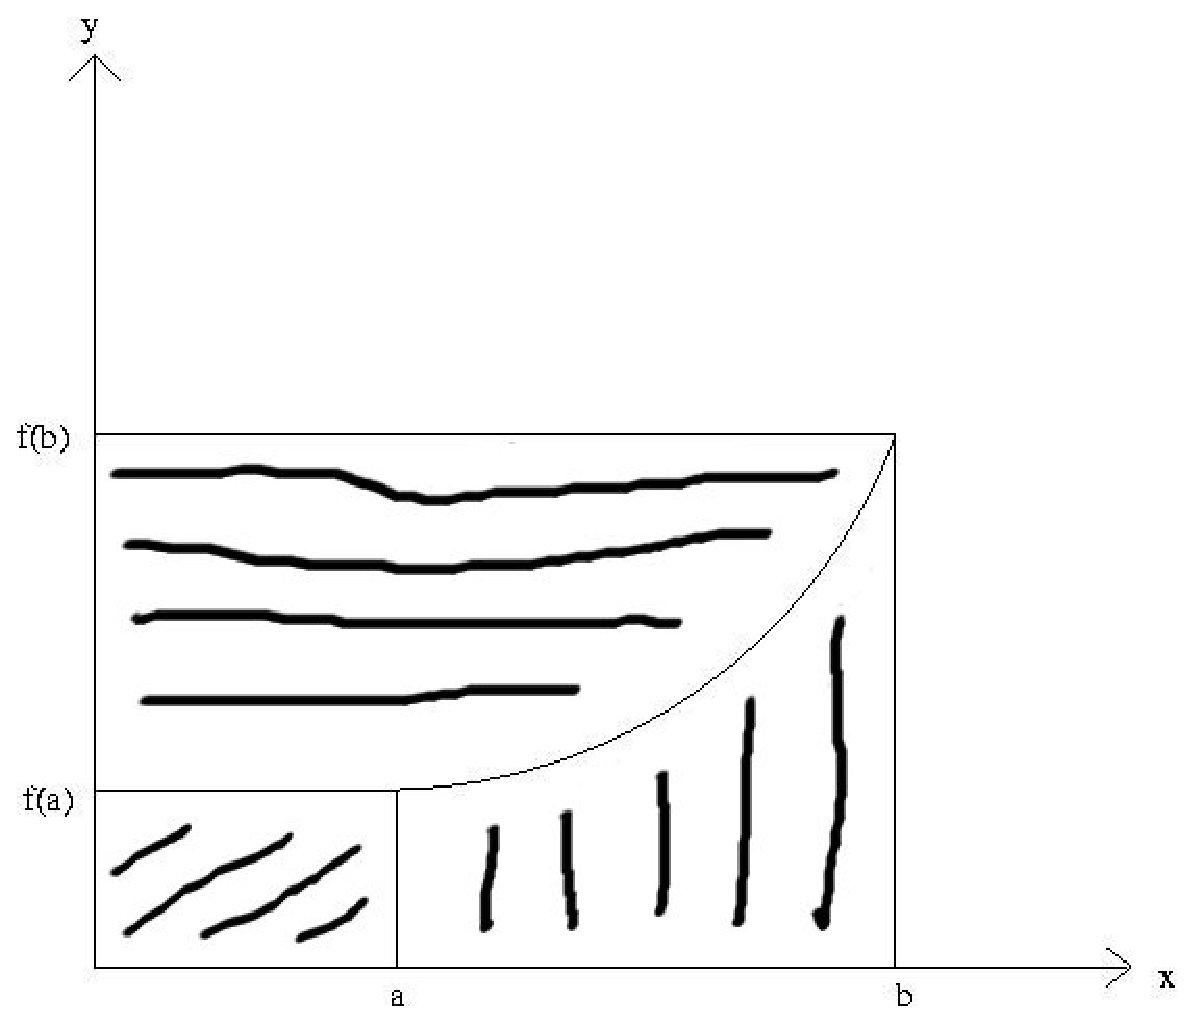
\epsfig{file=Figures/umkehr,scale=0.4}} 
  \caption{Die Funktion $f:[a,b] \rightarrow\mathbb{R}$}
  \label{fig:umkehr.eps}
\end{figure}

Ersetzen wir in dieser Gleichung  $b$ durch $x$ und stellen die Gleichung nach dem ersten
Integral um, so erhalten wir
\begin{equation}
  \label{eq:umkehr}
  \int_a^x f(t)\, \dr t = x\cdot f(x) - a\cdot f(a) - \int_{f(a)}^{f(x)} g(t)\, \dr t 
\end{equation}
Sind wir nur an Stamm-Funktionen interessiert, so k\"onnen wir den konstanten Term $a\cdot f(a)$
weglassen.  Dann schreibt sich die letzte Gleichung als
\begin{equation}
  \label{eq:umkehr1}
  \int f(x)\, \dr x = x\cdot f(x) - G\bigl(f(x)\bigr) \quad \mbox{mit}\;\; G(x) := \int g(x)\, \dr x. 
\end{equation}

\example 
Wir betrachten die Funktion $f(x) = \ln(x)$ mit der Umkehr-Funktion 
$g(x) = \exp(x)$.  Wegen $\ds\int \exp(x)\,\dr x = \exp(x)$ gilt 
\\[0.3cm]
\hspace*{1.3cm}
$\bint \ln(x) = x\cdot \ln(x) - \exp\bigl(\ln(x)\bigr) = x\cdot \ln(x) - x$. \eox

\subsection{Berechnung der Fl\"ache eines Kreises}
Wir zeigen, wie sich der Fl\"achen-Inhalt eines Kreises berechnen l\"asst.  Ein Kreis vom Radius 1 kann
nach dem Satz des Pythagoras  in der Koordinaten-Ebene durch die Relation $x^2 + y^2 = 1$ dargestellt werden.
L\"osen wir diese Gleichung nach $x$ auf, so wird der Kreis durch die beiden Funktionen $x
\mapsto \sqrt{1 - x^2}$
und $x \mapsto -\sqrt{1 - x^2}$ f\"ur $x\in[-1,1]$ beschrieben.  Wir beschr\"anken
uns nun auf den Viertelkreis im ersten Quadranten der Koordinaten-Ebene.  Die Fl\"ache
dieses Viertelkreises ist durch das Integral 
\\[0.2cm]
\hspace*{1.3cm}
$I := \dint{0}{1} \sqrt{1 - x^2\,}\, \dr x$
\\[0.2cm]
gegeben, welches wir nun berechnen.  Zun\"achst f\"uhren wir die Koordinaten-Transformation
$x = \sin(t)$ durch.  Dann erhalten wir
\\[0.2cm]
\hspace*{1.3cm}
$\ds\frac{\dr x}{\dr t} = \cos(t)$, \quad also $\dr x = \cos(t)\cdot \dr t$.
\\[0.2cm]
Wegen $0=\sin(0)$ und $1 = \sin(\pi/2)$ haben wir
\\[0.2cm]
\hspace*{1.3cm}
$\ds I = \int_0^{\frac{\pi}{2}} \sqrt{1 - \sin^2(t)\,} \cdot \cos(t)\, \dr t = \int_0^{\frac{\pi}{2}} \cos(t) \cdot \cos(t)\, \dr t$.
\\[0.2cm]
Dieses Integral versuchen wir nun mit partieller Integration zu vereinfachen.  Wir setzen
in Gleichung \ref{eq:partInt0} $u'(t) := \cos(t)$ und $v(t) = \cos(t)$.  Wegen $u(t) = \sin(t)$ und $v'(t) = -\sin(t)$ erhalten wir dann
\\[0.2cm]
\hspace*{1.3cm}
$\ds I = \sin(t)\cdot \cos(t)\bigg|_0^{\frac{\pi}{2}} + \int_0^{\frac{\pi}{2}}\sin(t)\cdot\sin(t)\,\dr t
   = \int_0^{\frac{\pi}{2}}\sin^2(t)\,\dr t$
\\[0.2cm]
Damit haben wir jetzt 
\\[0.2cm]
\hspace*{1.3cm}
$\ds I = \int_0^{\frac{\pi}{2}}\cos^2(t)\,\dr t =  \int_0^{\frac{\pi}{2}}\sin^2(t)\,\dr t$
\\[0.2cm]
Daraus folgt \\
\hspace*{1.3cm}
$
\begin{array}[t]{llcl}
\Leftrightarrow & 2\cdot I & = & \ds \int_0^{\frac{\pi}{2}}\cos^2(t)\,\dr t + \int_0^{\frac{\pi}{2}}\sin^2(t)\,\dr t \\[0.5cm]
\Leftrightarrow & 2\cdot I & = & \ds \int_0^{\frac{\pi}{2}}\bigl(\cos^2(t) + \sin^2(t)\bigr)\,\dr t \\[0.5cm]
\Leftrightarrow & 2\cdot I & = & \ds \int_0^{\frac{\pi}{2}} 1 \,\dr t \\[0.5cm]
\Leftrightarrow & 2\cdot I & = & \ds t\; \Big|_0^{\frac{\pi}{2}}  \\[0.4cm]
\Leftrightarrow & 2\cdot I & = & \ds \frac{\pi}{2}  \\[0.4cm]
\Leftrightarrow & I & = & \ds \frac{\pi}{4}
\end{array}
$
\\[0.3cm]
Damit haben wir f\"ur die Fl\"ache eines Viertelkreises den Wert $\ds\frac{\pi}{4}$ gefunden, der
ganze Kreis hat also die Fl\"ache $\pi$.

\section{Berechnung der Bogenl\"ange}
Gelegentlich tritt das Problem auf, die L\"ange der Strecke zu berechnen, die durch einen
Funktions-Graphen beschrieben wird.  Geht es darum, die Bogenl\"ange des Graphen der Funktion 
$f:[a,b] \rightarrow\mathbb{R}$ in dem Intervall $[a,b]$ zu berechnen, so zerlegen wir das
Intervall in $[a,b]$ in $n$ Teilintervalle der L\"ange 
\\[0.2cm]
\hspace*{1.3cm}
$\ds h = \frac{b - a}{n}$.
\\[0.2cm]
Das Teilst\"uck des Graphen, das sich von dem Punkt $\bigl\langle x, f(x) \bigr\rangle$  bis zu dem Punkt 
$\bigl\langle x + h, f(x+h) \bigr\rangle$ erstreckt, kann f\"ur kleine Werte von $h$ n\"aherungsweise
durch die Sekante von dem  Punkt $\bigl\langle x, f(x) \bigr\rangle$  zu dem Punkt
$\bigl\langle x + h, f(x+h) \bigr\rangle$  approximiert werden.  Nach dem Satz des
Pythagoras hat diese Sekante die L\"ange
\\[0.2cm]
\hspace*{1.3cm}
$ds = \sqrt{h^2 + \bigl(f(x+h) - f(x)\bigr)^2\,}$.
\\[0.2cm] 
Nach Definition der Ableitung von $f$ gilt f\"ur kleine Werte von $h$
\\[0.2cm]
\hspace*{1.3cm}
$\ds \frac{f(x+h) - f(x)}{h} \approx f'(x)$.
\\[0.2cm]
Also haben wir 
\\[0.2cm]
\hspace*{1.3cm}
$f(x+h) - f(x) \approx f'(x) \cdot h$.
\\[0.2cm]
Setzen wir diesen Wert in der obigen Formel f\"ur ein, so erhalten wir
\\[0.2cm]
\hspace*{1.3cm}
$\ds ds \approx \sqrt{h^2 + \bigl(f'(x) \cdot h\bigr)^2\,} = h \cdot \sqrt{1 + \Bigl(\frac{\mathrm{d}\/f}{\dr x}\Bigr)^2\,}$.
\\[0.2cm]
Die L\"ange $l$ des gesamten Funktions-Graphen erhalten wir, wenn wir diesen Ausdruck von $a$ bis $b$
aufintegrieren: 
\\[0.2cm]
\hspace*{1.3cm}
\colorbox{red}{\colorbox{orange}{\framebox{$\ds l = \dint{a}{b} \sqrt{1 + \Bigl(\frac{\dr f}{\dr x}\Bigr)^2\,} \dr x$}}}

\example
Wir berechnen die L\"ange $l$ des Kreisbogens, der durch die Funktion $f:[0,1] \rightarrow\mathbb{R}$ mit
\\[0.2cm]
\hspace*{1.3cm}
$f(x) = \sqrt{1 - x^2}$
\\[0.2cm]
definiert ist.  Anschaulich sollte diese L\"ange ein Viertel des Umfangs eines Kreises mit Radius $1$ betragen.
Es gilt
\\[0.2cm]
\hspace*{1.3cm}
$\ds\frac{\mathrm{d}\/f}{\dr x} = \frac{1}{2} \cdot \frac{-2 \cdot x}{\sqrt{1 - x^2}} = 
                  \frac{- x}{\sqrt{1 - x^2}}
$.
\\[0.2cm]
Also haben wir f\"ur die L\"ange
\\[0.2cm]
\hspace*{1.3cm}
$
\begin{array}[t]{lcl}
l & = & \dint{0}{1} \sqrt{1 + \frac{x^2}{1 - x^2}\,}\, \dr x \\[0.5cm]
  & = & \dint{0}{1} \frac{1}{\sqrt{1 - x^2\,}}\, \dr x
\end{array}
$
\\[0.2cm]
An dieser Stelle wenden wir die Substitutions-Regel
\\[0.2cm]
\hspace*{1.3cm}
$\dint{a}{b} f'(x) \cdot  g\bigl(f(x)\bigr)\, \dr x = \dint{f(a)}{f(b)} g(x)\, \dr x$
\\[0.2cm]
an, wobei wir 
\\[0.2cm]
\hspace*{1.3cm}
$f(x) := \sin(x)$,\quad $g(x) := \ds \frac{1}{\sqrt{1 - x^2\,}}$, 
\quad $a := 0$ \quad und \quad $b := \ds \frac{\pi}{2}$
\\[0.2cm]
setzen. Wegen
\\[0.2cm]
\hspace*{1.3cm}
$f'(x) = \cos(x)$, \quad $\sin(0) = 0$ \quad und \quad $\sin(\pi/2) = 1$
\\[0.2cm]
folgt dann
\\[0.2cm]
\hspace*{1.3cm}
$
\begin{array}[t]{lcl}
l & = & \dint{0}{\pi/2} \cos(x) \cdot \frac{1}{\sqrt{1 - \sin^2(x)}}\, \dr x  \\[0.6cm]
  & = & \dint{0}{\pi/2} \cos(x) \cdot \frac{1}{\cos(x)}\, \dr x  \\[0.6cm]
  & = & \dint{0}{\pi/2} 1\, \dr x  \\[0.6cm]
  & = &  x \Bigl|_0^{\pi/2}  \\[0.4cm]
  & = & \ds \frac{\pi}{2}  
\end{array}
$
\\[0.2cm]
und das ist genau der Umfang eines Viertel-Kreises. \eod

\exercise
Berechnen Sie die Bogenl\"ange der Parabel $x \mapsto x^2$ im Intervall $[0,1]$. 

\hint
Diese Aufgabe ist zwar etwas anspruchsvoller, aber daf\"ur ist die L\"osung umso lehrreicher.  Es ist
sinnvoll, die L\"osung in die folgenden Schritte aufzuteilen:
\begin{enumerate}[(a)]
\item Zun\"achst definieren wir die beiden Funktionen $\sinh(x)$ (lese: \emph{Sinus Hyperbolicus}) und
      $\cosh(x)$ (lese: \emph{Cosinus Hyperbolicus}) wie folgt:
      \\[0.2cm]
      \hspace*{1.3cm}
      $\ds\sinh(x) = \frac{1}{2} \cdot \bigl(e^x - e^{-x}\bigr)$ \quad und \quad
      $\ds\cosh(x) = \frac{1}{2} \cdot \bigl(e^x + e^{-x}\bigr)$. 
\item Die Umkehrfunktion der Funktion $x \mapsto \sinh(x)$ k\"onnen Sie auf den nat\"urlichen
      Logarithmus zur\"uck f\"uhren, indem Sie die Gleichung
      \\[0.2cm]
      \hspace*{1.3cm}
      $y = \frac{1}{2} \cdot \bigl(e^x - e^{-x}\bigr)$
      \\[0.2cm]
      nach $x$ aufl\"osen.  Setzen Sie zun\"achst $\alpha := e^x$, so erhalten Sie eine quadratische
      Gleichung f\"ur $\alpha$ in Abh\"angigkeit von $y$.  Wenn Sie aus dieser Gleichung $\alpha$
      berechnet haben, dann finden Sie anschlie{\ss}end $x$ nach der Formel $x = \ln(\alpha)$.

      Die Umkehrfunktion, die wir auf diesem Weg berechnet haben, ist als 
      \href{https://de.wikipedia.org/wiki/Areasinus_Hyperbolicus_und_Areakosinus_Hyperbolicus}{\emph{Areasinus Hyperbolicus}}
      bekannt und wird von uns als $\mathtt{arsinh}(x)$ geschrieben.  In der angels\"achsischen
      Literatur findet sich auch die Schreibweise $\sinh^{-1}(x)$ f\"ur diese Funktion.
\item Dann zeigen wir
      \\[0.2cm]
      \hspace*{1.3cm}
      $\df\; \sinh(x) = \cosh(x)$ \quad und \quad $\df\; \cosh(x) = \sinh(x)$.
\item Weiter zeigen wir durch rein algebraische Umformungen, dass
      \\[0.2cm]
      \hspace*{1.3cm}
      $1 + \sinh^2(x) = \cosh^2(x)$
      \\[0.2cm]
      f\"ur alle $x\in \mathbb{R}$ gilt.
\item Nun berechnen wir das Integral
      \\[0.2cm]
      \hspace*{1.3cm}
      $\ds I(x) := \int_0^x \cosh^2(t)\, \dr t$
      \\[0.2cm]
      mit Hilfe einer partiellen Integration, wobei wir im Verlaufe der Rechnung an geeigneter
      Stelle die Identit\"at $\cosh^2(x) = 1 + \sinh^2(x)$ ber\"ucksichtigen. 
\item Das bei der Berechnung der Bogenl\"ange der Parabel auftretende Integral kann nun vermittels einer
      Substitution auf das Integral $I(x)$ zur\"uck gef\"uhrt werden. \eod 
\end{enumerate}


\section{Uneigentliche Integrale}
Ist bei dem Ausdruck $\int_a^b f(x)\,\dr x$ die Funktion $f$ an einer der Intervall-Grenzen
nicht definiert, so bezeichnen wir den Ausdruck als \blue{uneigentliches Integral.}  Wir
betrachten nur den Fall, dass die Funktion $f$ nur in dem halboffenen Intervall $(a, b]$
definiert ist, w\"ahrend $f$  in dem Punkt $a$ nicht definiert sein soll.  Beispielsweise
ist die Funktion $x \mapsto \frac{1}{\sqrt{x}}$ im Punkt $x=0$ nicht definiert.  In diesem
Fall definieren wir 
\\[0.2cm]
\hspace*{1.3cm}
$\ds \int_a^b f(x)\, \dr x := \lim\limits_{h\rightarrow 0 \atop h > 0} \int_{a+h}^b f(x)\, \dr x$.
\\[0.2cm]
Wir betrachten als Beispiel das Integral der Funktion $\ds x \mapsto \frac{1}{\sqrt{x}}$ in
dem Intervall $[0,1]$.  Es gilt
\\[0.2cm]
\hspace*{1.3cm}
$\ds \int_0^1 \frac{1}{\sqrt{x}}\, \dr x 
 = \lim\limits_{h\rightarrow 0 \atop h >  0} \int_{h}^1 \frac{1}{\sqrt{x}}\, \dr x
 = \lim\limits_{h\rightarrow 0 \atop h >  0} 2\cdot\sqrt{x}\; \Big|_h^1
 = \lim\limits_{h\rightarrow 0 \atop h >  0} 2\cdot\sqrt{1} - 2\cdot\sqrt{h} = 2$.
\\[0.2cm]
Ein anderer Fall liegt vor, wenn eine der Integrations-Grenzen den Wert Unendlich hat.
Wir betrachten nur den Fall $b= \infty$.  In diesem Fall definieren wir
\\[0.2cm]
\hspace*{1.3cm}
$\ds \int_a^\infty f(t)\, \dr t := \lim\limits_{x\rightarrow \infty} \int_{a}^x f(t)\, \dr t$.
\\[0.2cm]
Wir betrachten als Beispiel die Funktion $\ds x \mapsto \frac{1}{x^2}$ in dem Intervall
$[1,\infty)$. Es gilt
\\[0.2cm]
\hspace*{1.3cm}
$\ds \int_1^\infty \frac{1}{t^2}\, \dr t = 
\lim\limits_{x\rightarrow \infty} \int_{1}^x \frac{1}{t^2}\, \dr t =
\lim\limits_{x\rightarrow \infty} - \frac{1}{t}\;\Big|_1^x =
\lim\limits_{x\rightarrow \infty} - \frac{1}{x} + \frac{1}{1}  = 1
$.
\\[0.2cm]
Indem wir Reihen und uneigentliche Integrale in Beziehung setzen, k\"onnen wir unter
Umst\"anden leicht sehen, dass eine Reihe konvergiert, denn es gilt der folgende Satz.


\begin{Satz}[Integral-Vergleichskriterium]
Es sei $f:[1,\infty) \rightarrow\mathbb{R}_+$ eine monoton fallende Funktion.  Dann gilt
\\[0.2cm]
\hspace*{1.3cm}
\colorbox{red}{\colorbox{orange}{\framebox{$\ds \lim\limits_{n \rightarrow \infty} \sum\limits_{i=1}^n f(i)$ existiert \quad g.d.w. \quad
$\ds \lim\limits_{x \rightarrow \infty} \int\limits_1^x f(t)\,\dr t$ existiert.}}}
\end{Satz}

\noindent
\textbf{Beweis}:
F\"ur alle $i\in \mathbb{N}$ mit $i>1$ und alle $x \in [i-1,i]$ gelten die Ungleichungen
\\[0.2cm]
\hspace*{1.3cm}
$i-1 \leq x$ \quad und \quad $x \leq i$.
\\[0.2cm]
Da die Funktion $f$ monoton fallend ist, folgt daraus
\\[0.2cm]
\hspace*{1.3cm}
$f(i) \leq f(x)$ \quad und \quad $f(x) \leq f(i-1)$.
\\[0.2cm]
Aus der Monotonie des Integral-Operators folgt nun
\\[0.2cm]
\hspace*{1.3cm}
$\ds\int\limits_{i-1}^{i} f(i)\, \dr x \leq \int\limits_{i-1}^{i} f(x)\, \dr x$
\quad und \quad
$\ds \int\limits_{i-1}^i f(x)\, \dr x \leq \int\limits_{i-1}^i f(i-1)\, \dr x$
\\[0.2cm]
Das Integral \"uber die konstanten Funktionen $x \mapsto f(i)$ bzw.~$x \mapsto f(i-1)$
liefert nur den konstanten Funktions-Wert multipliziert mit der L\"ange des Intervalls, die nat\"urlich 1
ist.  Also haben wir die Ungleichungen
\\[0.2cm]
\hspace*{1.3cm}
$\ds f(i) \leq \int\limits_{i-1}^{i} f(x)\, \dr x$
\quad und \quad
$\ds\int_{i-1}^{i} f(x)\, \dr x \leq f(i\!-\!1)$
\\[0.2cm]
gezeigt.  Summieren wir diese Ungleichungen f\"ur alle $i$ aus der Menge $\{2,\cdots,n\}$,
  so erhalten wir 
\\[0.2cm]
\hspace*{1.3cm}
$\ds\sum\limits_{i=2}^n f(i) \leq \dint{1}{n} f(x)\, \dr x$
\quad und \quad
$\dint{1}{n} f(x)\, \dr x \leq \sum\limits_{i=2}^n f(i\!-\!1)$
\\[0.2cm]
Bei der ersten Ungleichung addieren wir noch $f(1)$, bei der zweiten Ungleichung ersetzen
wir die Summations-Variable $i$ durch $i+1$ und erhalten:
\\[0.2cm]
\hspace*{1.3cm}
$\ds \sum\limits_{i=1}^n f(i) \leq f(1) + \dint{1}{n} f(x)\, \dr x$
\quad und \quad
$\dint{1}{n} f(x)\, \dr x \leq \sum\limits_{i=1}^{n-1} f(i)$
\\[0.2cm]
Falls nun das Integral $\int\limits_{1}^\infty f(x)\, \dr x$ existiert, so gilt
\\[0.2cm]
\hspace*{1.3cm}
$\ds \sum\limits_{i=1}^{n} f(i) \leq f(1) + \int\limits_{1}^n f(x)\, \dr x \leq f(1) + \int\limits_{1}^\infty f(x)\, \dr x$
\\[0.2cm]
Damit ist dann die Folge 
\\
\hspace*{1.3cm}
$\ds \biggl(\sum\limits_{i=1}^{n}  f(i)\biggr)_{n\in\mathbb{N}}$ 
\\ 
monoton und beschr\"ankt, folglich konvergent.  Existiert umgekehrt der Grenzwert
$\ds \sum\limits_{i=1}^{\infty} f(i)$, so  ist aufgrund der zweiten Ungleichung auch die Folge
\\[0.3cm]
\hspace*{1.3cm}
$\ds \biggl(\int_{1}^n f(x)\, \dr x\biggr)_{n\in\mathbb{N}}$
\\[0.3cm]
beschr\"ankt.  Da diese Folge au{\ss}erdem monoton ist, folgt die Konvergenz. \hspace*{\fill} $\Box$
\vspace*{0.3cm}

\noindent
\textbf{Beispiel}: Wir betrachten das Integral 
\\[0.2cm]
\hspace*{1.3cm}
$\ds I(\alpha) := \int\limits_{1}^\infty \frac{1}{t^\alpha}\, \dr t$ \quad f\"ur $\alpha > 0$.
\\[0.2cm]
Falls $\alpha \not= 1$ ist,  gilt 
\\[0.2cm]
\hspace*{1.3cm}
$
\begin{array}[t]{clcl}  
  &I(\alpha) & = & \ds \int_{1}^\infty \frac{1}{t^\alpha}\, \dr t  \\[0.3cm]
= & \ds \lim\limits_{x \rightarrow \infty} \int_1^x \frac{1}{t^\alpha}\, \dr t 
& = & \ds \lim\limits_{x \rightarrow \infty} \frac{t^{1-\alpha}}{1-\alpha} \,\bigg|_1^x \\[0.5cm]
= & \ds \lim\limits_{x \rightarrow \infty} \frac{x^{1-\alpha}-1}{1-\alpha}.
\end{array}
$
\\[0.3cm]
Im Falle $\alpha = 1$ haben wir
\\[0.2cm]
\hspace*{1.3cm}
$I(\alpha) = \ln(x)$.
\\[0.2cm]
Nun h\"angt alles davon ab, ob $\alpha < 1$, $\alpha = 1$ oder 
 $\alpha > 1$ ist.
\begin{enumerate}
\item Falls $\alpha < 1$ ist, haben wir $1-\alpha>0$ und damit gilt
      \\[0.2cm]
      \hspace*{1.3cm}
      $\ds I(\alpha) = \lim\limits_{x \rightarrow \infty} \frac{x^{1-\alpha}-1}{1-\alpha} = \infty$
      \\[0.2cm]
      Also konvergiert die Summe 
      \\[0.2cm]
      \hspace*{1.3cm}
      $\ds \sum\limits_{i=1}^{\infty} \frac{1}{i^\alpha}$
      \\[0.2cm]
      in diesem Fall nicht.
\item Falls $\alpha = 1$ ist, gilt
      \\[0.2cm]
      \hspace*{1.3cm}
      $I(1) = \lim\limits_{x \rightarrow \infty} \dint{1}{x}\; \frac{1}{t}\, \dr t 
            =  \lim\limits_{x \rightarrow \infty} \ln(x)  = \infty
      $
      \\[0.2cm]
      Im letzten Schritt haben wir hier ausgenutzt, dass
      \\[0.2cm]
      \hspace*{1.3cm}
      $\lim\limits_{x \rightarrow \infty} \ln(x) = \infty$
      \\[0.2cm]
      gilt.  Das folgt daraus, dass die Funktion $x \mapsto \ln(x)$ einerseits monoton steigend ist und
      dass andererseits 
      \\[0.2cm]
      \hspace*{1.3cm}
      $\ln\bigl(\exp(n)\bigr) = n$ \quad f\"ur alle $n \in \mathbb{N}$  
      \\[0.2cm]
      gilt, denn die letzte Gleichung zeigt, dass die Funktion $x \mapsto \ln(x)$ beliebig gro{\ss} wird. 

      Insgesamt k\"onnen wir nun aus dem Integral-Vergleichskriterium folgern, dass die
      harmonische Reihe divergiert:
      \\[0.2cm]
      \hspace*{1.3cm}
      $\ds\sum\limits_{i=1}^{\infty} \frac{1}{i} = \infty$.
\item Falls $\alpha > 1$ ist, haben wir $1-\alpha<0$ und damit gilt
      \\[0.2cm]
      \hspace*{1.3cm}
      $\ds I(\alpha) = \lim\limits_{x \rightarrow \infty} \frac{x^{1-\alpha}-1}{1-\alpha} = \frac{1}{\alpha-1}$
      \\[0.2cm]
      In diesem Fall konvergiert also die Summe 
      \\[0.2cm]
      \hspace*{1.3cm}
      $\ds \sum\limits_{i=1}^{\infty} \frac{1}{i^\alpha}$.
\end{enumerate}

\exercise
Untersuchen Sie mit Hilfe des Integral-Vergleichskriteriums, ob die
Reihe 
\\[0.2cm]
\hspace*{1.3cm}
$\ds \sum\limits_{n=1}^\infty \frac{1}{n\cdot (n+1)}$ 
\qquad
konvergiert.  \eox


\section{Numerische Integration$^*$}
Die Gleichung $x = \cos(x)$ haben wir zwar numerisch l\"osen k\"onnen, aber wir waren nicht in
der Lage, einen algebraischen Ausdruck f\"ur die L\"osung anzugeben.  Auch bei der Integration
von Funktionen ist es nicht immer m\"oglich, einen algebraischen Ausdruck f\"ur die
Stamm-Funktion einer Funktion anzugeben.  Beispielsweise konnte Liouville 
(\href{https://de.wikipedia.org/wiki/Joseph_Liouville}{Joseph Liouville}, 1809 -- 1882) beweisen, dass das
unbestimmte Integral
\\[0.2cm]
\hspace*{1.3cm}
$\ds\int \exp(-x^2)\, \dr x$
\\[0.2cm]
nicht auf die uns bisher bekannten Funktionen zur\"uck gef\"uhrt werden kann \cite{rosenlicht:72}.  F\"ur die
praktische Berechnung von Integralen ben\"otigen wir daher numerische Methoden.

\subsection{Die Trapez-Regel$^*$}
Die wohl naheliegenste Methode besteht darin, die zu integrierende Funktion st\"uckweise
linear zu interpolieren und dann das zur berechnende Integral durch das Integral der
st\"uckweise linearen Funktion zu approximieren.
Ist das Integral $\int_a^b f(t)\,\dr t$ zu berechnen, so wird zun\"achst das Intervall $[a,b]$
in $n$ gleich gro{\ss}e Teilintervalle zerlegt.  Das $i$-te Teilintervall ist $[a+(i-1)\cdot h,
a+i\cdot h]$ mit $h := \frac{b-a}{n}$ und $i=1,\cdots,n$.
Wir setzen $x_i := a+i\cdot h$.
Innerhalb des $i$-ten Teilintervalls wird die Funktion $f(x)$ dann durch die Gerade 
\\[0.2cm]
\hspace*{1.3cm}
$\ds g(x) = f\bigl(x_{i-1}\bigr)\cdot \frac{x - x_i}{x_{i-1} - x_i} + f\bigl(x_{i}\bigr)\cdot \frac{x - x_{i-1}}{x_{i} - x_{i-1}}$
\\[0.2cm]
approximiert.  Das Integral \"uber $g(x)$ im Intervall $[x_{i-1}, x_i]$ ist dann
$$
\begin{array}[t]{cl}
  &  \dint{x_{i-1}}{x_i} g(x)\, \dr x \\[0.5cm]
= &  \dint{x_{i-1}}{x_i} f\bigl(x_{i-1}\bigr)\cdot \frac{x - x_i}{x_{i-1} - x_i} + f\bigl(x_{i}\bigr)\cdot \frac{x - x_{i-1}}{x_{i} - x_{i-1}}\,\dr x \\[0.5cm]
= &  \ds\frac{f\bigl(x_{i-1}\bigr)}{x_{i-1} - x_i} \cdot  \int_{x_{i-1}}^{x_i} (x - x_i)\,\dr x +
                  \frac{f\bigl(x_{i}\bigr)}{x_{i} - x_{i-1}} \cdot  \int_{x_{i-1}}^{x_i} (x - x_{i-1})\,\dr x \\[0.5cm]
= &  \ds\frac{f\bigl(x_{i-1}\bigr)}{x_{i-1} - x_i} \cdot \frac{1}{2} \cdot (x - x_i)^2 \Big|_{x_{i-1}}^{x_i}  +
                  \frac{f\bigl(x_{i}\bigr)}{x_{i} - x_{i-1}} \cdot \frac{1}{2} \cdot (x - x_{i-1})^2 \Big|_{x_{i-1}}^{x_i} \\[0.5cm]
= &  \ds-\frac{f\bigl(x_{i-1}\bigr)}{x_{i-1} - x_i} \cdot \frac{1}{2} \cdot (x_{i-1} - x_i)^2   +
                   \frac{f\bigl(x_{i}\bigr)}{x_{i} - x_{i-1}} \cdot \frac{1}{2} \cdot (x_i - x_{i-1})^2  \\[0.5cm]
= &  \ds \frac{1}{2} \cdot f\bigl(x_{i-1}\bigr) \cdot (x_i - x_{i-1}) +
     \frac{1}{2} \cdot f\bigl(x_{i}\bigr)   \cdot (x_i - x_{i-1})    \\[0.5cm]
= &  \ds \frac{1}{2} \cdot  \Bigl(f\bigl(x_{i}\bigr) + f\bigl(x_{i-1}\bigr)\Bigr) \cdot  (x_{i} - x_{i-1}) 
\end{array}
$$
Die letzte Formel l\"asst sich geometrisch deuten, denn der Ausdruck 
\\[0.2cm]
\hspace*{1.3cm}
$\frac{1}{2} \cdot  \bigl(f(x_{i}) + f(x_{i-1})\bigr) \cdot  (x_{i} - x_{i-1})$
\\[0.2cm]
beschreibt gerade die Fl\"ache eines Trapezes mit der Breite $h = x_i - x_{i-1}$ und  Seiten
der L\"ange $f(x_i)$ und $f(x_{i-1})$. Daher wird dieses Verfahren zur Berechnung eines Integrals auch als 
\emph{Trapez-Regel} bezeichnet.
Um das Integral \"uber das gesamte Intervall $[a,b]$ zu berechnen,
m\"ussen wir die Integrale \"uber die einzelnen Intervalle lediglich aufsummieren.  Wir erhalten dann 
$$
\begin{array}[t]{lcl}
 \dint{a}{b} f(x)\,\dr x & \approx & \ds
       \sum\limits_{i=1}^n \frac{1}{2} \cdot \bigl(f(x_i) + f(x_{i-1})\bigr) \cdot (x_i-x_{i-1})  
       \\[0.5cm]
 & = & \ds
       \sum\limits_{i=1}^n \frac{1}{2} \cdot \bigl(f(a+i\cdot h) + f(a+(i-1)\cdot h)\bigr) \cdot  h  \\[0.5cm]
 & = & \ds
       \biggl(\frac{1}{2}\cdot f(a) \;+\; \sum\limits_{i=1}^{n-1} f\Bigl(a+i\cdot \frac{b-a}{n}\Bigr)\;+\;\frac{1}{2}\cdot f(b)\biggr) \cdot  \frac{b-a}{n}  \\[0.5cm]
\end{array}
$$
Abbildung \ref{fig:trapezoidal.eps} auf Seite \pageref{fig:trapezoidal.eps} zeigt die
numerische Berechnung des Integrals $\int_0^1 \exp(x^2)\,\dr x $ mit Hilfe der Trapez-Regel.
In diesem Fall ist $n=3$.
F\"uhren wir die Berechnung tats\"achlich aus, so erhalten wir die N\"aherung 
\\[0.2cm]
\hspace*{1.3cm}
$\dint{0}{1} \exp(-x^2)\,\dr x \approx 0.7399864752\cdots$.
\\[0.2cm]
Der exakte Wert ist $0.7468241328$, unter Ber\"ucksichtigung der Tatsache, dass wir $n=3$
gew\"ahlt haben ist die N\"aherung also gar nicht so schlecht.   Erh\"ohen wir $n$ auf den Wert 
$300$, so erhalten wir mit der Trapez-Regel die N\"aherung $0.7468234519$, der Fehler ist
dann also kleiner als $10^{-6}$.  Im n\"achsten Satz geben wir eine theoretische Analyse des
Fehlers.

\begin{figure}[!h]
  \centering
   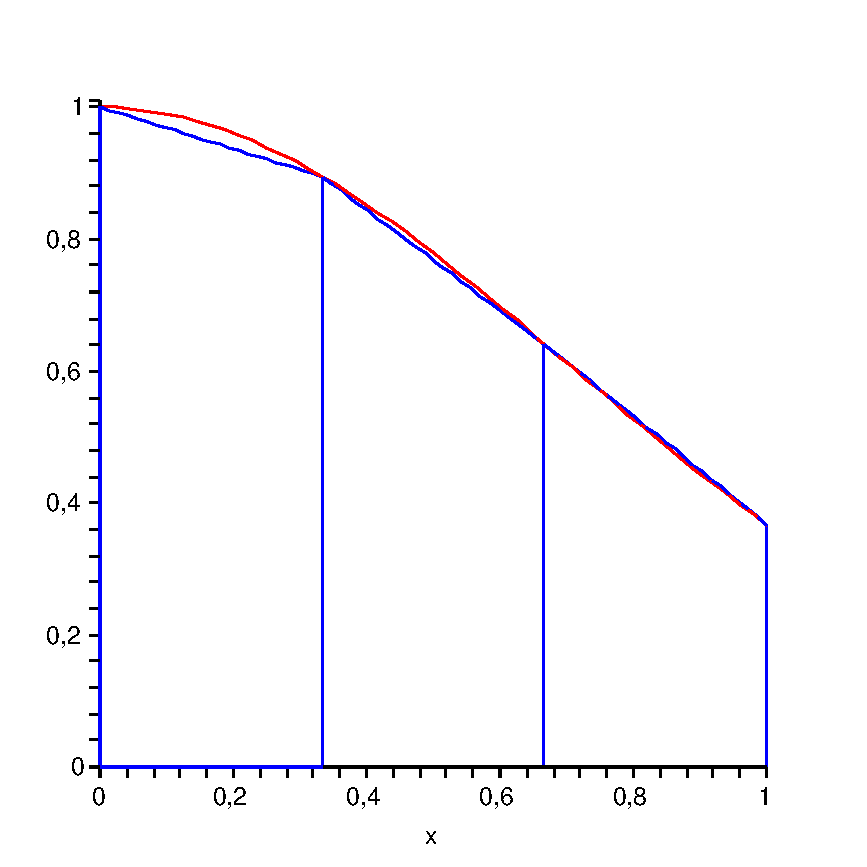
\epsfig{file=Figures/trapezoidal.eps,scale=0.6}
   \caption{Berechnung des Integrals  $\int_0^1 \exp(-x^2)\, \dr x$ mit Hilfe der Trapez-Regel.}
  \label{fig:trapezoidal.eps}
\end{figure}

\begin{Satz}
  Ist die Funktion $f:[a,b]\rightarrow \mathbb{R}$ zweimal differenzierbar, gilt
  \\[0.2cm]
  \hspace*{1.3cm}
  $\bigl|f^{(2)}(x)\bigr| \leq K$ \quad f\"ur alle $x\in[a,b]$
  \\[0.2cm]
  und definieren wir gem\"a{\ss} der Trapez-Regel 
  \\[0.2cm]
  \hspace*{1.3cm}
  $\ds I_{\mbox{\scriptsize Trapez}} := \biggl(\frac{1}{2}\cdot f(a) \;+\; \sum\limits_{i=1}^{n-1} f\Bigl(a+i\cdot \frac{b-a}{n}\Bigr)\;+\;\frac{1}{2}\cdot f(b)\biggr) \cdot  \frac{b-a}{n}$
  \\[0.2cm]
  so kann der Unterschied zwischen dem exakten Integral und der N\"aherung $I_{\mbox{\scriptsize Trapez}}$
  wie folgt abgesch\"atzt werden:
  \\[0.2cm]
  \hspace*{1.3cm}
  $\ds \left| \int_a^b f(x)\,\dr x - I_{\mbox{\scriptsize Trapez}} \right| \;\leq\; 
   \frac{K}{12}\cdot  \frac{(b-a)^3}{n^2}$
\end{Satz}

\noindent
\textbf{Beweis}: Bei der Ableitung der Trapez-Regel haben wir $f(x)$ durch ein lineares
Polynom interpoliert.  Nach Satz \ref{satz:interpolationsFehler} gilt f\"ur den Unterschied
zwischen $f(x)$ und dem interpolierenden Polynom $p(x)$ vom Grad $n$
\\[0.2cm]
\hspace*{1.3cm}
  $\ds f(x) - p(x) = \frac{f^{(n+1)}(\xi)}{(n+1)!} \cdot  \prod\limits_{i=0}^{n}(x-x_i)$.
\\[0.2cm]
Dabei ist $\xi$ ein nicht n\"aher bekannter Wert aus dem Intervall $[a,b]$.
Bei linearer Interpolation ist $n=1$ und also haben wir
\\[0.2cm]
\hspace*{1.3cm}
  $\ds f(x) - p(x) = \frac{f^{(2)}(\xi)}{2} \cdot  (x-x_{i-1})\cdot (x-x_i)$.
\\[0.2cm]
Aufgrund der Voraussetzung \"uber die zweite Ableitung von $f(x)$ haben wir also
\begin{equation}
  \label{eq:intError1}
  |f(x) - p(x)| \leq \frac{K}{2} \cdot  |(x-x_{i-1})\cdot (x-x_i)|  
\end{equation}
In dem Intervall $[x_{i-1},x_i]$ gilt $x-x_{i-1} \geq 0$ und $x-x_i \leq 0$,
also haben wir
\\[0.2cm]
\hspace*{1.3cm}
 $|(x-x_{i-1})\cdot (x-x_i)| = -(x-x_{i-1})\cdot (x-x_i)$.
\\[0.2cm]
Integrieren wir die Ungleichung \ref{eq:intError1} in dem Intervall $[x_{i-1},x_i]$, so
erhalten wir 
\\[0.3cm]
\hspace*{1.3cm}
$
\begin{array}[t]{cl}
      & \ds  \left|\int_{x_{i-1}}^{x_i} f(x)\,\dr x - \int_{x_{i-1}}^{x_i}p(x)\,\dr x\right| \\[0.5cm]
 \leq & \ds  \int_{x_{i-1}}^{x_i} \bigl|f(x)\,\dr x - p(x)\bigr|\,\dr x \\[0.5cm]
 \leq & \ds \frac{K}{2} \cdot  \int_{x_{i-1}}^{x_i} \bigl|(x-x_{i-1})\cdot (x-x_i)\bigr|\,\dr x  \\[0.5cm]
 \leq & \ds -\frac{K}{2} \cdot  \int_{x_{i-1}}^{x_i} (x-x_{i-1})\cdot (x-x_i)\,\dr x  \\[0.5cm]
 =    & \ds -\frac{K}{2} \cdot  \frac{-1}{6} \cdot  (x_i-x_{i-1})^3\\[0.3cm]
 =    & \ds \frac{K}{12} \cdot  (x_i-x_{i-1})^3
\end{array}
$
\\[0.2cm]
Diese Ungleichung gilt nun f\"ur jedes $i=1,\cdots,n$.  Summieren wir diese Ungleichungen
f\"ur alle Intervalle auf, so erhalten wir 
\\[0.2cm]
\hspace*{1.3cm}
$
\begin{array}[t]{lcl}  
\ds \left| \int_a^b f(x)\,\dr x - I_{\mbox{\scriptsize Trapez}} \right|
& \leq & \ds \sum\limits_{i=1}^n \frac{K}{12} \cdot  (x_i-x_{i-1})^3 \\[0.5cm]
& \leq & \ds \sum\limits_{i=1}^n \frac{K}{12} \cdot  \Bigl(\frac{b-a}{n}\Bigr)^3 \\[0.5cm]
& \leq & \ds n \cdot  \frac{K}{12} \cdot  \Bigl(\frac{b-a}{n}\Bigr)^3  \\[0.5cm]
& \leq & \ds \frac{K}{12} \cdot  \frac{(b-a)^3}{n^2} \\[0.5cm]
\end{array}
$
\\[0.2cm]
Falls wir also die Zahl der Intervalle verzehnfachen, sinkt der Fehler auf ein Hundertstel.
\hspace*{\fill} $\Box$
\vspace*{0.3cm}

\exercise
Berechnen Sie, in wieviele Teilintervalle das Intervall $[0,1]$
aufgeteilt werden muss, wenn das Integral
\\[0.2cm]
\hspace*{1.3cm}
$\ds \int_0^1 e^{-x^2}\, \dr x$
\\[0.2cm]
mit Hilfe der Trapez-Regel mit einer Genauigkeit von $10^{-6}$ berechnet werden soll. \eod


\subsection{Die Simpson'sche Regel$^*$}
Anstatt die zu integrierende Funktion $f$ durch ein lineares Polynom zu interpolieren,
k\"onnen wir $f$ auch durch ein Polynom zweiten Grades interpolieren.  Wir brauchen dann
nat\"urlich drei St\"utzstellen. Daher integrieren wir jetzt nicht mehr \"uber ein Intervall
$[x_{i-1},x_i]$, sondern nehmen stattdessen das Intervall $[x_{i-1},x_{i+1}]$ und
benutzen $x_{i-1}$, $x_i$ und $x_{i+1}$ als St\"utzstellen.
Die Funktion $f(x)$ approximieren wir in dem Intervall mit der Methode von Lagrange nach
der Formel
\\[0.2cm]
\hspace*{1.3cm}
$
\begin{array}[t]{lcl}
p(x) & = & \ds f(x_{i-1})\cdot \frac{(x-x_i)\cdot (x-x_{i+1})}{(x_{i-1}-x_i)\cdot (x_{i-1}-x_{i+1})}  \\[0.5cm]
     & + & \ds f(x_{i})\cdot \frac{(x-x_{i-1})\cdot (x-x_{i+1})}{(x_{i}-x_{i-1})\cdot (x_{i}-x_{i+1})}  \\[0.5cm]
     & + & \ds f(x_{i+1})\cdot \frac{(x-x_{i-1})\cdot (x-x_{i})}{(x_{i+1}-x_{i-1})\cdot (x_{i+1}-x_{i})}
\end{array}$
\\[0.2cm]
Setzen wir hier $x_{i-1}= x_i-h$ und $x_{i+1}= x_i+h$ und
integrieren dann $p(x)$ in dem Intervall $[x_{i}-h,x_{i}+h]$, so erhalten wir mit Hilfe von \textsl{SymPy} das Ergebnis 
% x[i-1] := x[i] - h;
% x[i+1] := x[i] + h;
% p(x) := f[i-1] * (x - x[i])   * (x - x[i+1]) / ( (x[i-1] - x[i]  ) * (x[i-1] - x[i+1]) ) +
%         f[i]   * (x - x[i-1]) * (x - x[i+1]) / ( (x[i]   - x[i-1]) * (x[i]   - x[i+1]) ) +
%         f[i+1] * (x - x[i-1]) * (x - x[i])   / ( (x[i+1] - x[i-1]) * (x[i+1] - x[i]  ) );
% IntKeppler := int( p(x), x = x[i-1] .. x[[i+1] );
\\[0.2cm]
\hspace*{1.3cm}
$\ds \int_{x_{i-1}}^{x_{i+1}} p(x)\,\dr x = \frac{1}{6}\cdot \bigl(f(x_{i-1}) + 4 \cdot  f(x_i) + f(x_{i+1})\bigr)\cdot (x_{i+1}-x_{i-1})$
\\[0.2cm]
Unterteilen wir das Intervall $[a,b]$ lediglich in zwei Teilintervalle $[a,\frac{a+b}{2}]$
und $[\frac{a+b}{2},b]$, so k\"onnen wir die obige Formel direkt verwenden.  Wir erhalten
dann die \emph{Kepler'sche Fassregel} (Johannes Kepler, 1571 -- 1630).
\begin{equation}
  \label{eq:keplerFass}
  \int_a^b f(x)\,\dr x \approx \frac{1}{6} \cdot \Bigl( f(a) + 4 \cdot f\Bigl(\frac{a+b}{2}\Bigr) + f(b)\Bigr)\cdot (b-a)
\end{equation}
Berechnen wir das Integral $\int_0^1 \exp(-x^2)\, \dr x$ mit dieser Regel, so erhalten wir 
$0.7471804290$ und der Fehler ist bereits kleiner als $4 \cdot 10^{-4}$.

Unterteilen wir das Intervall $[a,b]$ in $n$ Intervalle und ist dar\"uber hinaus $n$ eine
gerade Zahl, so k\"onnen wir die Regel \ref{eq:keplerFass} jeweils auf die beiden  benachbarten
Intervalle $[x_{2\cdot i},x_{2\cdot i+1}]$ und $[x_{2\cdot i+1},x_{2\cdot i+2}]$ anwenden,
wobei der Index $i$ \"uber alle Elemente der Menge $\{0,\cdots,(n-1)/2\}$ l\"auft.
Setzen wir $h:=\frac{b-a}{n}$ und $x_i := a + i\cdot h$, so erhalten wir
die Formel 
\begin{equation}
  \label{eq:intSimpson}  
\begin{array}[t]{lcl}
 \ds \int_a^b f(x)\,\dr x 
& \approx & \ds\frac{h}{3}\cdot \sum\limits_{i=0}^{(n-1)/2} \Bigl( f(x_{2\cdot i}) + 4\cdot f(x_{2\cdot i+1}) + f(x_{2\cdot i+2}) \Bigr) \\[0.3cm]
& = & \ds\frac{h}{3}\cdot \biggl(f(x_0) \;+\; 4\cdot \sum\limits_{i=0}^{(n-1)/2} f(x_{2\cdot i+1}) \;+\;
                                                          2\cdot \sum\limits_{i=1}^{(n-1)/2} f(x_{2\cdot i}) \;+\; f(x_n)\biggr) \\[0.3cm]
\end{array}
\end{equation}
Die obige Formel tr\"agt den Namen Simpson'sche Regel (Thomas Simpson, 1710 -- 1761).
Falls die Funktion $f$ insgesamt viermal differenzierbar ist und falls dar\"uber hinaus 
die vierte Ableitung von $f$ der Ungleichung 
\\[0.2cm]
\hspace*{1.3cm}
$|f^{(4)}(x)| \leq K$
\\[0.2cm]
gen\"ugt, so l\"asst sich der Fehler, der bei der Verwendung der Simpson'schen Regel entsteht, durch
\\[0.2cm]
\hspace*{1.3cm}
$\ds\frac{K}{180}\cdot \frac{(b-a)^5}{n^4}$
\\[0.2cm]
absch\"atzen.  Verdoppeln wir die Zahl $n$ der Intervalle, so verkleinert sich der Fehler
also um das 16-fache! W\"ahlen wir beispielsweise $n=20$ und berechnen das Integral
$\int_0^1 \exp(-x^2)\, \dr x$, so erhalten wir den Wert
$0.746824183$ und der Fehler ist kleiner als $10^{-7}$.
\vspace*{0.3cm}


\exercise
\begin{enumerate}[(a)]
\item Berechnen Sie mit Hilfe der Kepler'schen Fass-Regel eine Approximation 
      f\"ur das Integral 
      \\[0.2cm]
      \hspace*{1.3cm}$\ds \int_0^{\frac{1}2} \sin(x)\, \dr x$.
\item Geben Sie eine m\"oglichst genaue Absch\"atzung f\"ur den Approximations-Fehler.
\item Vergleichen Sie ihr Ergebnis mit dem exakten Wert. \eod
\end{enumerate}
\pagebreak

\exercise
Gegenstand dieser Aufgabe ist die numerische Berechnung der Summe
\\[0.2cm]
\hspace*{1.3cm}
 $\ds \sum\limits_{k=1}^\infty \frac{1}{k^2}$.
\\[0.2cm]
Gehen  Sie zur Berechnung dieser Summe in folgenden Schritten vor.
\begin{enumerate}[(a)]
\item Approximieren Sie die Rest-Summe $\ds\sum\limits_{k=n}^\infty \frac{1}{k^2}$ 
      durch ein geeignetes Integral.

      \textbf{Hinweis}: Es gilt $\ds f(k) = \int_{k-\frac{1}{2}}^{k+\frac{1}{2}} f(k) \, \dr t \approx \int_{k-\frac{1}{2}}^{k+\frac{1}{2}} f(t) \, \dr t$.
\item Berechnen Sie eine obere Absch\"atzung f\"ur den Approximations-Fehler,
      den Sie bei der Integration in Teil (a) erhalten.
      
      \textbf{Hinweis}: Sch\"atzen Sie die auftretenden Summen durch Integrale nach oben ab.
\item Berechnen Sie, wir gro{\ss} Sie $n$ w\"ahlen m\"ussen, damit der Approximations-Fehler
      kleiner als $10^{-6}$ bleibt.
\item Geben Sie nun einen N\"aherungs-Wert f\"ur die Summe $\ds\sum\limits_{k=1}^\infty \frac{1}{k^2}$ an,
      der sich von dem exakten \\[-0.2cm]
      Ergebnis um weniger als $10^{-6}$ unterscheidet.
\end{enumerate}



%%% Local Variables: 
%%% mode: latex
%%% TeX-master: "analysis"
%%% End: 
